% !TEX TS-program = pdflatex
% !TEX encoding = UTF-8 Unicode

% This is a simple template for a LaTeX document using the "article" class.
% See "book", "report", "letter" for other types of document.

\documentclass[11pt,twoside]{report} % use larger type; default would be 10pt

\linespread{1}
\renewcommand*\rmdefault{ptm}

\usepackage[utf8]{inputenc} % set input encoding (not needed with XeLaTeX)

\usepackage{placeins}

%%% Examples of Article customizations
% These packages are optional, depending whether you want the features they provide.
% See the LaTeX Companion or other references for full information.

%%% PAGE DIMENSIONS
\usepackage{geometry} % to change the page dimensions
\geometry{a4paper} % or letterpaper (US) or a5paper or....
\geometry{
	margin=2.5cm,
} % for example, change the margins to 2 inches all round
% \geometry{landscape} % set up the page for landscape
%   read geometry.pdf for detailed page layout information

\usepackage{graphicx} % support the \includegraphics command and options

% \usepackage[parfill]{parskip} % Activate to begin paragraphs with an empty line rather than an indent

\usepackage[explicit]{titlesec}

%%% PACKAGES
\usepackage{url}
\usepackage{booktabs} % for much better looking tables
\usepackage{array} % for better arrays (eg matrices) in maths
\usepackage{paralist} % very flexible & customisable lists (eg. enumerate/itemize, etc.)
\usepackage{verbatim} % adds environment for commenting out blocks of text & for better verbatim
\usepackage[final]{pdfpages}
\usepackage{pdflscape}
\usepackage{rotating}
\usepackage{rotfloat}
\usepackage{wrapfig}
\usepackage{hyperref}
\usepackage[official]{eurosym}
\usepackage{graphicx}
\usepackage{caption}
\usepackage{subcaption}
\usepackage{units}
\usepackage{longtable}
\usepackage{multirow}
% These packages are all incorporated in the memoir class to one degree or another...

%%% HEADERS & FOOTERS
\usepackage{fancyhdr} % This should be set AFTER setting up the page geometry
\pagestyle{fancy} % options: empty , plain , fancy
\renewcommand{\headrulewidth}{0pt} % customise the layout...
\lhead{\small A Recipe for Making Homemade Tagliatelle}\chead{}\rhead{\small Boshuizen, Van den Enk, De Jonge}
\lfoot[\small \today]{\small \thepage}
\cfoot{}
\rfoot[\small \thepage]{\small \today}


\newcommand*\Hidechapter{%
\titleformat{\chapter}[display]
  {}{}{0pt}{\Huge}
}

\newcommand*\Hide{%
\titleformat{\chapter}[display]
  {}{}{0pt}{\Huge}
\titleformat{\chapter}
  {}{}{0pt}{}
}

%%% SECTION TITLE APPEARANCE
\usepackage{sectsty}
\allsectionsfont{\sffamily\mdseries\upshape} % (See the fntguide.pdf for font help)
% (This matches ConTeXt defaults)

%%% RULE

\newcommand{\HRule}{\rule{\linewidth}{0.5mm}}

%%% BIBLIOGRAPHY

\usepackage{apacite}                           %bibliography in apa-style

%%% ToC (table of contents) APPEARANCE
\usepackage[nottoc,notlof,notlot]{tocbibind} % Put the bibliography in the ToC
\usepackage[titles,subfigure]{tocloft} % Alter the style of the Table of Contents
\renewcommand{\cftsecfont}{\rmfamily\mdseries\upshape}
\renewcommand{\cftsecpagefont}{\rmfamily\mdseries\upshape} % No bold!

\setcounter{secnumdepth}{3}

%%% TABLES

\renewcommand{\arraystretch}{1.2}

\usepackage{afterpage}

\newcommand\blankpage{%
    \null
    \thispagestyle{empty}%
    \newpage}

%%% END Article customizations

%%% The "real" document content comes below...

\begin{document}

\begin{titlepage}

\begin{center}


% Upper part of the page

\includegraphics[width=1\textwidth]{./logo}\\[1cm]    

\textsc{\Large Research Proposal}\\[0.5cm]

% Title
\HRule \\[0.4cm]
{ \huge \bfseries Flashmaps: integrating concept maps with flashcards}\\[0.4cm]

\HRule \\[1.5cm]

% Author and supervisor
\begin{minipage}{0.4\textwidth}
\begin{flushleft} \large
\emph{Author:}\\
Micha \textsc{van den Enk} {[}s1004654{]} \\
\end{flushleft}
\end{minipage}
\begin{minipage}{0.4\textwidth}
\begin{flushright} \large
\emph{Supervisors:} \\
Dr. A.H. \textsc{Gijlers} \\
Dr. L. \textsc{Bollen} \\
\end{flushright}
\end{minipage}

\vfill

% Bottom of the page
Word count: 3440

{\large April 20, 2016}

\end{center}

\end{titlepage}

\afterpage{\blankpage}

\setcounter{tocdepth}{1}
\tableofcontents
\thispagestyle{fancy}
\newpage

\chapter{Summary}

In literature, a distinction is often made between meaningful encoding and rote learning in terms of retrieval practices, of which the former is regarded to be more beneficial than the latter. A prominent example of meaningful encoding is the concept map, where retrieval practice is often used by means of flashcards. However, recently studies have indicated the importance of both aspects. Because of this, a new tool is developed, attempting to bridge the gap between meaningless rote memorisation and meaningful learning by combining the active retrieval mechanisms of flashcards with the meaningful visualisation by concept maps. In the proposed research, the effects of flashmaps will be investigated in terms of the learning effects measured by learning gain, and the affective effects measured by a questionnaire. Furthermore, the use of the tool will be investigated by means of interviews and user logs. The research will take place within a Dutch classroom setting by first measuring prior knowledge with a pre-test, then letting the students use the tool for 7 days and finally measuring their final knowledge with a post-test. Finally, a sample of the students will be interviewed. This research hopefully leads to a better way of meaningful rote memorisation and gains more insight in how flashcard systems and concept maps can benefit from each other.

\chapter{Project Description}

\section{Problem Statement}

%Describe a rationale for the focus and aim of this study; why is the topic of your research important? This can be done from a theoretical, as well as from a practical point of view (or both). For example, what gaps exist in current literature, what problems need to be solved, What tool/intervention do we need, what societal changes have led to a need for this research?

%IDEAL AFFAIRS

%Within the history of educational psychology, three major distinct perspectives of the learning process have been proposed, namely the behavioural, the cognitive and the constructivist perspective \cite{ertmer}. Learning theory first shifted from behaviourist models to cognitivist models, resulting in a change in focus on observable performance to what is happening within the learner itself. However, both these theories still assume a primarily objectivistic world view, whereas the final perspective of constructivism offer an alternative, relativistic world view. Within this model, the student is not supplied with information, but instead has to construct his own model of reality. \citeA{glaserfield} however criticised constructivism for its lack of rote memorisation, and argues for a need to train students so that they permanently possess facts and are able to repeat them flawlessly whenever they are needed, while also understanding what is placed into their memory.

%introduction flashcards

%n1.1.7, n1.1.3

Both the taxonomy of learning by \citeA{bloom} as a revision of this taxonomy by \citeA{krathwohl}, as well as the three stages of skill acquisition by \citeA{skillacquisition}, propose that all learning should start with memorising factual knowledge. Furthermore, \citeA{glaserfield}, one of the main founders for critical constructivism, expresses a need for training students so that they permanently possess facts and are able to repeat them flawlessly whenever they are needed, while also understanding what is placed into their memory. \citeA{ltwm} adds to this by stating that in order to perform complex tasks, people must maintain access to large amounts of information, and that solely encoding knowledge is not sufficient. Despite this, \citeA{karpicke4} argues that "[r]etrieval processes, the processes involved in using available cues to actively reconstruct knowledge, have received less attention" (p. 158), whereas basic research on learning and memory has emphasised that retrieval must be considered in any analysis of learning. Therefore, this project aims to research a tool for meaningfully enhancing the retrieval process. 

\citeA{karpicke4} also states that meaningful learning often is defined in contrast to rote learning, and that active retrieval is thought of as an example of the latter leading to poorly organised knowledge that lacks coherence and integration. However, in another study they found active retrieval to enhance learning of meaningful educational materials and that these effects are long-lasting, not short-lived \cite{karpicke2}. In this study, he compared the effects of active retrieval using measures of meaningful learning contrasting to a popular learning strategy known as concept mapping. The latter involves a graph consisting of nodes representing concepts and labeled lines denoting the relation between a pair of nodes \cite{ruiz1} (see figure~\ref{fig:conceptmap}). Multiple researchers have found by means of both qualitative and quantitative studies that concept maps can promote meaningful learning leading to positive effects on students \cite{hwang2, subramaniam, canas}. This has been demonstrated in comparison to activities such as reading text passages, attending lectures, and participating in class discussions \cite{singh, nesbit2}. \citeA{canas} describes the process of concept mapping as the only effective way of using the concept map, which refers to students constructing their own concept maps. This is why the concept map is generally viewed as a tool in alignment with the constructivist perspective. Because of this, the concept map might seem as a solution to the need asked by \citeA{glaserfield} and his peers. However, the aforementioned article by \citeA{karpicke2} reveals that retrieval practices produced better performance than elaborative concept mapping for meaningful learning.

\begin{figure}
    \centering
    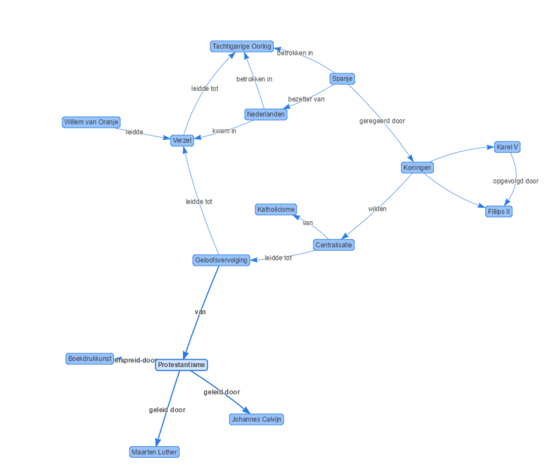
\includegraphics[width=\textwidth]{img/conceptmap}
    \caption{An example of a concept map}
    \label{fig:conceptmap}
\end{figure}

One of the currently existing methods for efficiently rote memorising information is the flashcard system, which entails studying declarative knowledge using active retrieval in a so-called paired-associate format. Within this format, learners are asked to associate terms with other terms outside meaning-focused tasks \cite{nakata}, for example by associating a definition with a presented concept. With flashcards, large numbers of words can be memorised in a very short time, and are more resistant to decay \cite{nakata, joseph}. Furthermore, when evaluating flashcards in a psychology setting, it was found that students who use flashcards have a significantly higher final average than those who do not \cite{burgess, golding}.

%EXPLAIN THE PROBLEM

%n1.1.2, n1.1.3.2, n1.1.3.8, n1.5.9, n1.2.1.2
Per contra, not all research favours using flashcards for textual comprehension. \citeA{zirkle} and \citeA{mccullough} state that flashcards are especially useful for learning declarative knowledge but not for textual comprehension. \citeA{zirkle} points out the overemphasis placed upon the rote memorisation of disconnected facts, whereas whatever it is that students are to place into memory they should, more importantly, understand. Furthermore, \citeA{hulstijn} describes flashcards as a relic of the old-fashioned behaviourist learning model, and states that we have to look for more modern constructivist models.

%EXPLAIN WHY THE PROBLEM IS IMPORTANT

%n1.1.1.7
Solving these problems could lead to better utilisation by teachers and students of producing a store of knowledge that remains flexibly retrievable, in contrast to only segregated paired associations which depend on specific cues in order to be retrieved. Furthermore, using computer-based flashcards have been used very widely \cite{nakata,burgess, golding,kornell}, and improving currently existing flashcards could reach a wide audience of future users of flashcard systems.

%PROPOSE A SOLUTION/IDEA AND ITS BENEFITS

%introduction concept maps

%n1.2.1, n1.(2.1),(1.3).1
% (Already covered above) An instructional tool more in line with constructivistic approaches is the concept map, which is a graph consisting of nodes representing concepts and labeled lines denoting the relation between a pair of nodes \cite{ruiz1} (see figure~\ref{fig:conceptmap}). Multiple researchers have found by means of both qualitative and quantitative studies that concept maps can promote meaningful learning leading to positive effects on students \cite{hwang2, subramaniam, canas}. This has been demonstrated in comparison to activities such as reading text passages, attending lectures, and participating in class discussions \cite{singh, nesbit2}. \citeA{canas} describes the process of concept mapping as the only effective way of using the concept map, which refers to students constructing their own concept maps. This is why the concept map is generally viewed as a tool in alignment with the constructivist perspective. Because of this, the concept map might seem as a solution to the need asked by \citeA{glaserfield} and his peers. However, a recent article by \citeA{karpicke2} reveals that paired associate learning produced better performance than elaborative concept mapping for meaningful learning, even on the short-term.


%introduction flashmaps

%n1.2.6.8 and n1.2.6.9 (Counterarguments), n1.2.5, n1.2.10
Therefore, another solution might be the development of a new tool, which will from henceforth be referred to as the flashmap system. The intention behind the flashmap system is to combine the paired associate mechanism of the flashcard system with the visual representation of the concept map, and is a new tool designed and developed for this research project. This tool might have the potential to bridge the gap between the two systems and therefore make meaningful and effective rote memorisation possible, for it makes the relations between the concepts explicit to the student and thereby increasing the organisation of the knowledge and reducing the segregation of facts. Thereby, it might provide a solution for the problems by \citeA{zirkle} described before.

For evaluating this flashmap system, a group of Dutch high school teachers of the Stedelijk Lyceum has been found willing to participate, with their students using either the flashmap or the flashcard system for self study parallel with classroom instruction. The content of the instruction will be the history of Dutch literature during the sixteenth and seventeenth century. For example, the students have to learn what the influence is of the Dutch War of Independence on the \emph{Spaanschen Brabander} by Bredero. Because of the content existing mainly of concepts with meaningful relations it fits to the concept map technique and thereby the flashmap system could be significantly beneficial over the flashcard system.

%SUMMARISE, END WITH RESEARCH GOALS

In conclusion, flashcards systems are an effective tool for meaningful learning, but could be enhanced by visualising it with concept maps, and therefore the effects of using a flashmap system over using a flashcard system will be investigated. 

\section{Theoretical Conceptual Framework}

%Describe theoretical framework where you introduce the most important concepts in your study and their relation

\subsection{Flashcards systems}

%n1.1.6, n1.1.1.8.6.1, n1.1.1.3.8.2
The most straightforward example of a flashcard system is a deck of physical cards, with on one side a question and on the other side an answer. Every day, the student has to go through the deck trying to answer the question on the card and checking his answer. If the answer is correct the card will be repeated the next day, and if incorrect it will be repeated the same day. The main disadvantage of this system is that it becomes time-intensive when more flashcards are introduced, because the student has to go through all of the cards every day. Because of this, newer systems relying on spaced repetition were introduced, with which the time intervals between repetitions increase every time the student answers correctly \citeA{microlearning}. It was found that systems using adaptive algorithms was more effective and more satisfactory to the user than the other strategies \cite{microlearning}.

The effects of flashcards have mainly been attributed to the spacing effect \cite{nakata, microlearning}, which means that repeated items are better remembered when both occurrences are separated by other events or items than when they are presented in immediate succession \cite{verkoeijen, logan, siegel, xue, karpicke2}.

\subsection{Concept maps}

%n1.2.4, n1.2.8
%According to \citeA{eppler}, a concept map is a hierarchical graph showing the relationships between concepts, including cross connections among concepts and their manifestations. The edges contain labels describing the relation between the concepts. They compare the concept map to several different other visual mapping techniques, which are the mind map, the conceptual diagram and the visual metaphor. A mind map is multicoloured and image-centred, is radial and represents semantic or other connections between portions of learned material hierarchically. The benefit of constructing a mind map is that it has a higher memorability than a concept map, but is more difficult to understand by others \cite{eppler}. The conceptual diagram entails abstract concepts in pre-defined category boxes with specified relationships, typically based on a theory or model. This diagram is more suitablefor analysing topics or situations through a proven analytic framework, however they have only a medium memorability and medium understandability by others. Finally, a visual metaphor is a praphic structure using the shape and elements of a familiar artiefact, activity, or story to organise content meaningfully and use the associations with the metaphor to convey additional meaning about the content. This technique is the most meaningful, memorable and understandable in comparison to the other technique, however it has a very limited extensibility \cite{eppler}.

According to \citeA{eppler}, concept maps are defined as hierarchical graphs showing the relationships between concepts, including cross connections among concepts and their manifestations. They also define them by differentiating them from other available visual mapping techniques - mind maps, conceptual diagrams and visual metaphors - by several factors. The function of a concept map is to show systematic relationships among sub-concepts relating to one main concept, without the need for a proven analytic framework or picture. This makes it easy to apply in classroom teaching and self study and a useful support tool for summarising key course topics. The main topic should be placed at the top, so the hierarchy of the concepts is conveyed intuitively. All concepts are represented by boxes or bubbles with text, and the relations by labeled arrows. It is a flexible tool and has a high understandability by others compared to the other techniques. It however does not necessarily assist memorability, and it is not easy to apply by novices and requires extensive training.

%1.2.6
%\citeA{canas} describes several conditions for using concept maps in learning: no conditions, focus question, root concept, list of concepts, restricting list of concepts, expert skeleton concept maps, concept mapping games, fill-in-the-Cmap and memorise the concept map. These concitions range from low to high scaffolding respectively. The no conditions condition asks students to create a concept map without any scaffolding. This often results in a descriptive instead of an explanatory map, and users are often intimidated and have difficulty constructing a concept map. A focus question helps student to create a more explanatory map by trying to answer specific questions. This has a positive effect on the quality of the resulting maps. A root concept provides the students with a minimum concept map containing the main topics, having a stronger effect than the focus question. The list of concepts condition entails that students get a list of concepts they can use for the construction of their map, resulting in better maps than under no conditions or when provided with a text including the topics. The restrincting list of concepts entails that the students are only allowed to use concepts from the list, which is an effective way of determining the student's prior knowledge. The expert skeleton map restricts the freedom of content and sturture, and overcomes the difficulty of students when getting started. Within coyncept mapping games students are iteratively provided with two concepts and are asked to label the links between them, this has proven to be both effective and affective. Filling in the cmap means that the students are provided with a concept map containing empty nodes which they have to fill in themselves. This technique is not recommended, because this is meant for rote learning purposes and not for meaningful learning. Finally, Memorising the concept map is not recommended for its lack of meaningful learning and integration with other relevant knowledge. It also undermines the need for learners to be actively engaged in assimilating new concepts and propositions into their cognitive structures.

\subsection{Flashmaps}

The flashmap is intended as an integration between the flashcard system and the concept map. The system uses a predefined concept map constructed by an expert which the users have to rote memorise. The concept map has the best combination of understandability and extensibility, whereas the low memorability is compensated by the flashcard system, and because it is predefined the construction difficulty is taken away. Where a flashcard system would then show a question, the flashmap shows a part of this concept map with one or more empty. The user then has to think of which concepts would fit in these nodes, and when requesting the answer the flashmaps shows the actual concepts. The student then can indicate per node whether he was right or not, which will then be used for rescheduling the nodes according to the adaptive algorithm (see figure~\ref{fig:flashmap}). \citeA{canas} describes that fill-in-the-cmap or memorise the concept map conditions are not recommended, because of the information in memorised concept maps not being integrated with other relevant knowledge and the lack of learners being actively engaged in assimilating new concepts and propositions into their cognitive structures. However, they do not provide statistics or literature in order to support this claim, and furthermore the findings from \citeA{karpicke2} about paired associate learning being more effective for meaningful learning than concept mapping puts this claim into doubt.

\begin{figure}
    \centering
    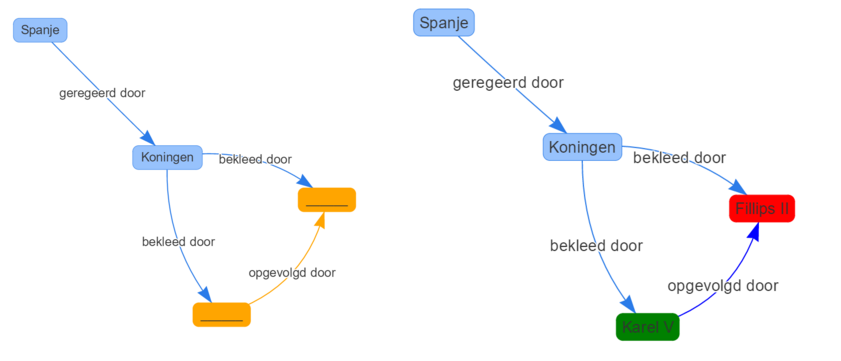
\includegraphics[width=\textwidth]{img/flashmap}
    \caption{A display of the flashmap system, where the user has to think of the concepts fitting in the orange nodes on the left, and has to indicate which nodes were correct on the right}
    \label{fig:flashmap}
\end{figure}

Finally, the flashmap creates the opportunity for a more interactive concept map that starts with a parsimonious and theme-oriented structure which gradually expand the details along with the instruction, which is hypothesised by \citeA{tzeng} to mitigate map shock. This phenomenon occurs when users view the kind of larger concept maps that might more fully capture textbook knowledge structures, but is a type of cognitive overload that prevents students from effectively processing the concept map and thereby inhibiting their ability to learn from it \cite{moore}. This mitigation will be facilitated by scheduling the central concepts towards the beginning and the details towards the end.

\section{Research Question and Model}
\newcounter{researchquestion}
\renewcommand{\theresearchquestion}{\Roman{researchquestion}}
\newcounter{subquestion}[researchquestion]
\renewcommand{\thesubquestion}{\alph{subquestion}}


%The research questions (hypotheses if applicable) and model are described here. A figure on your research model is optional.

For researching the effects of the flashmap system relative to the effects of the flashcard system, it is important to consider two main factors: its actual benefits (research question~\ref{benefits}\ref{effectiveness} and~\ref{efficiency}), and its perceived benefits (research question~\ref{perception}\ref{usefulness} and~\ref{ease}). Furthermore, for the validity of the system and of the experiment it is important to investigate how the system was used by the students (research question~\ref{howused}).

To research whether the flashmap system is more effective or efficient than the flashcard system, the learning gain of high school the students will be measured, referring to the knowledge obtained by a student over the course of an instruction. Sequentially, the efficiency of the system is determined by the learning gain controlled for time spend on the system.

For measuring the affectiveness of the systems, the Technology Acceptance Model by \citeA{tam} will be used (see figure~\ref{fig:tam}). This model predicts the use of an information system by measuring the Perceived Usefulness and the Perceived Ease of Use of the user. These variables are mediators between External Variables and Attitude toward using, leading to Behavioural intention to use, which in turn leads to the Actual system use.

Finally, for the answering the final question an interview will be conducted with a sample of the participants, and by the server logging usage information about the user.

\begin{figure}
    \centering
    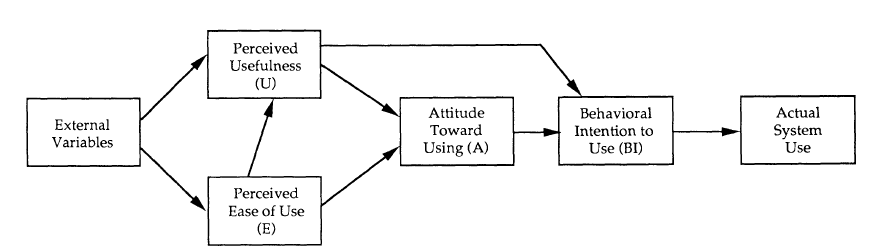
\includegraphics[width=\textwidth]{img/tam}
    \caption{The Technology Acceptance Model by \protect\citeA{tam}}
    \label{fig:tam}
\end{figure}

This leads to the following research questions: Regarding high school students learning for Dutch literature using the flashmap system in comparison to them using the flashcard system...

\refstepcounter{researchquestion}\label{benefit}
\refstepcounter{subquestion}\label{effectiveness}
\Roman{researchquestion}\alph{subquestion}. ...is the learning gain larger?

\refstepcounter{subquestion}\label{efficiency}
\Roman{researchquestion}\alph{subquestion}. ...is the learning gain larger controlled for the time spend with the system?

\refstepcounter{researchquestion}\label{perception}
\refstepcounter{subquestion}\label{usefulness}
\Roman{researchquestion}\alph{subquestion}. ...do they perceive the system to be more useful?

\refstepcounter{subquestion}\label{ease}
\Roman{researchquestion}\alph{subquestion}. ...do they perceive the system to be easier to use?

\refstepcounter{researchquestion}\label{howused}
\Roman{researchquestion} How did the students use the flashmap or flashcard system?

\section{Scientific and Practical Relevance}

%Describe the expected contribution of your study (how can scientists, practitioners benefit)
Answering the research questions has both practical and scientific relevance. From a practical perspective, it has potential to overcome the criticism from various authors about flashcard systems and answer the need for meaningful rote memorisation. From a scientific perspective, it could confirm the hypothesis by \citeA{tzeng} that an expanding concept map might mitigate map shock. It also makes way for new research opportunities, for example what the effect is of integrating the flashmap with the games condition formulated by \citeA{canas}. 

%n1.1.3.1
%n2.1

\chapter{Research Design and Methods}

\section{Research design}

%What kind of research is this? (e.g. exploratory, confirmatory, intervention-based, evaluationbased, design-based, etc.). Justify the type of research design(s) you intend to use :descriptive (e.g., case study) ;correlational (longitudinal) ; (quasi-)experimental; review etc.

Research questions \ref{benefit}\ref{effectiveness}, \ref{efficiency}, \ref{perception}\ref{usefulness} and \ref{ease} will be investigated using intervention-based research. Because of the systems being used for self-study by the students, they can be individually assigned to a condition, and this enables the use of a true experimental design. Since this will provide the most valid and reliable results, this research design is implemented in this experiment.

Furthermore, research question~\ref{howused} is a qualitative research question, and therefore an interview will take place after the experiment in order to investigate how the students used the system. Next to the interviews, user data and actions will be logged by the server.

The quantitative and qualitative results will be mixed for the purposes of triangulation and expansion as described by \citeA{mixedmethods}. The interviews and logs could provide insight in the degree of which the systems were used the intended way and in why students had certain perceptions on using the systems. Both triangulation and expansion will be on a partial level of mixing, will take place concurrently, and the quantitative data will be dominant, since the qualitative data exists only to triangulate and expand the quantitative data. 

\section{Respondents}

%This section is where you describe the who will be approached to participate in your study and how many. Explain how they will be selected (sampling method). Make sure this justification fits your research design and questions.

%1.5.4

100 15 to 17 year old tenth grade Dutch high school students will be approached. They already have to prepare themselves for an exam on the same topic and thereby have incentive to learn. To increase the response rate, the students will be rewarded with a \euro{} 5 voucher for participation. The participants will be assigned to either the flashcard or the flashmap condition at random.

\section{Instrumentation}

%Describe the instruments you will use; make a link between the research variables and the instruments explicit (operationalization process) and describe their measurement level if applicable. If you are using existing instruments, provide references.

%n1.5.6

The learning gain will be measured by the means of a pre- and post-test. Both tests will consist of random items from an item bank measuring both knowledge and comprehension levels of the students \cite{bloom}. The tests will be directly based on the concept map, and also will be evaluated by the teacher in order to increase its validity. By using an item bank, the tests will be comparable and thereby the learning gain can be determined by subtracting the score on the pre-test from that on the post-test. Finally, the controlled learning gain is calculated by dividing the learning gain by time spent on the software. The survey will be an adaptation of the standardised Technology Acceptance Model questionnaire \citeA{tamq}.

The interviews will be conducted using a topic list \cite{baarda}, including “frequency”, “usefulness”, “ease of use”, “external conditions”, and “attitudes”, based on the Technology Acceptance Model. The server logs will contain information about the reaction times, the correct responses, the nodes studied, the time investment, the IP address, and the client, which will be registered per user and per session.

\section{Procedure}

%Describe the procedure for your data collection; what will respondents in your study do? Here you can also address any constraints you may need to cope with in the research and the actions to guard its quality and validity. Potential ethical concerns can be addressed here too.

%n1.6

An outline of the procedure is given in figure~\ref{fig:procedure}.

Before the experiment takes place the experiment will have to be approved by the ethics committee from the University of Twente. On approval, the students and their parents will be briefed by means of a letter, which consists out of a general description, conditions (voluntary participation and withdrawal at all times), and rewards. They will also both be asked to fill in an informed consent form.

After that, the students with consent will be provided with a general introduction on flashcards by both the teacher and the researcher within the classroom. Then, when the students log into the system for the first time, the server assigns them randomly to either the flashcard or the flashmap condition. By making the introduction ambiguous enough, the students will not be able to recognise this condition in order to guarantee a double-blind experiment.

Before they start using the system they will be asked for general descriptive information such as date of birth and gender. A code will be assigned to them making it only able for the teacher to determine their identity. After that the pre-test follows, and for the next week will use the system daily for fifteen minutes. Finally the post-test and survey will be conducted. At the end of the post-test, the students can also indicate whether they are willing to participate in the interview.

\begin{figure}
    \centering
    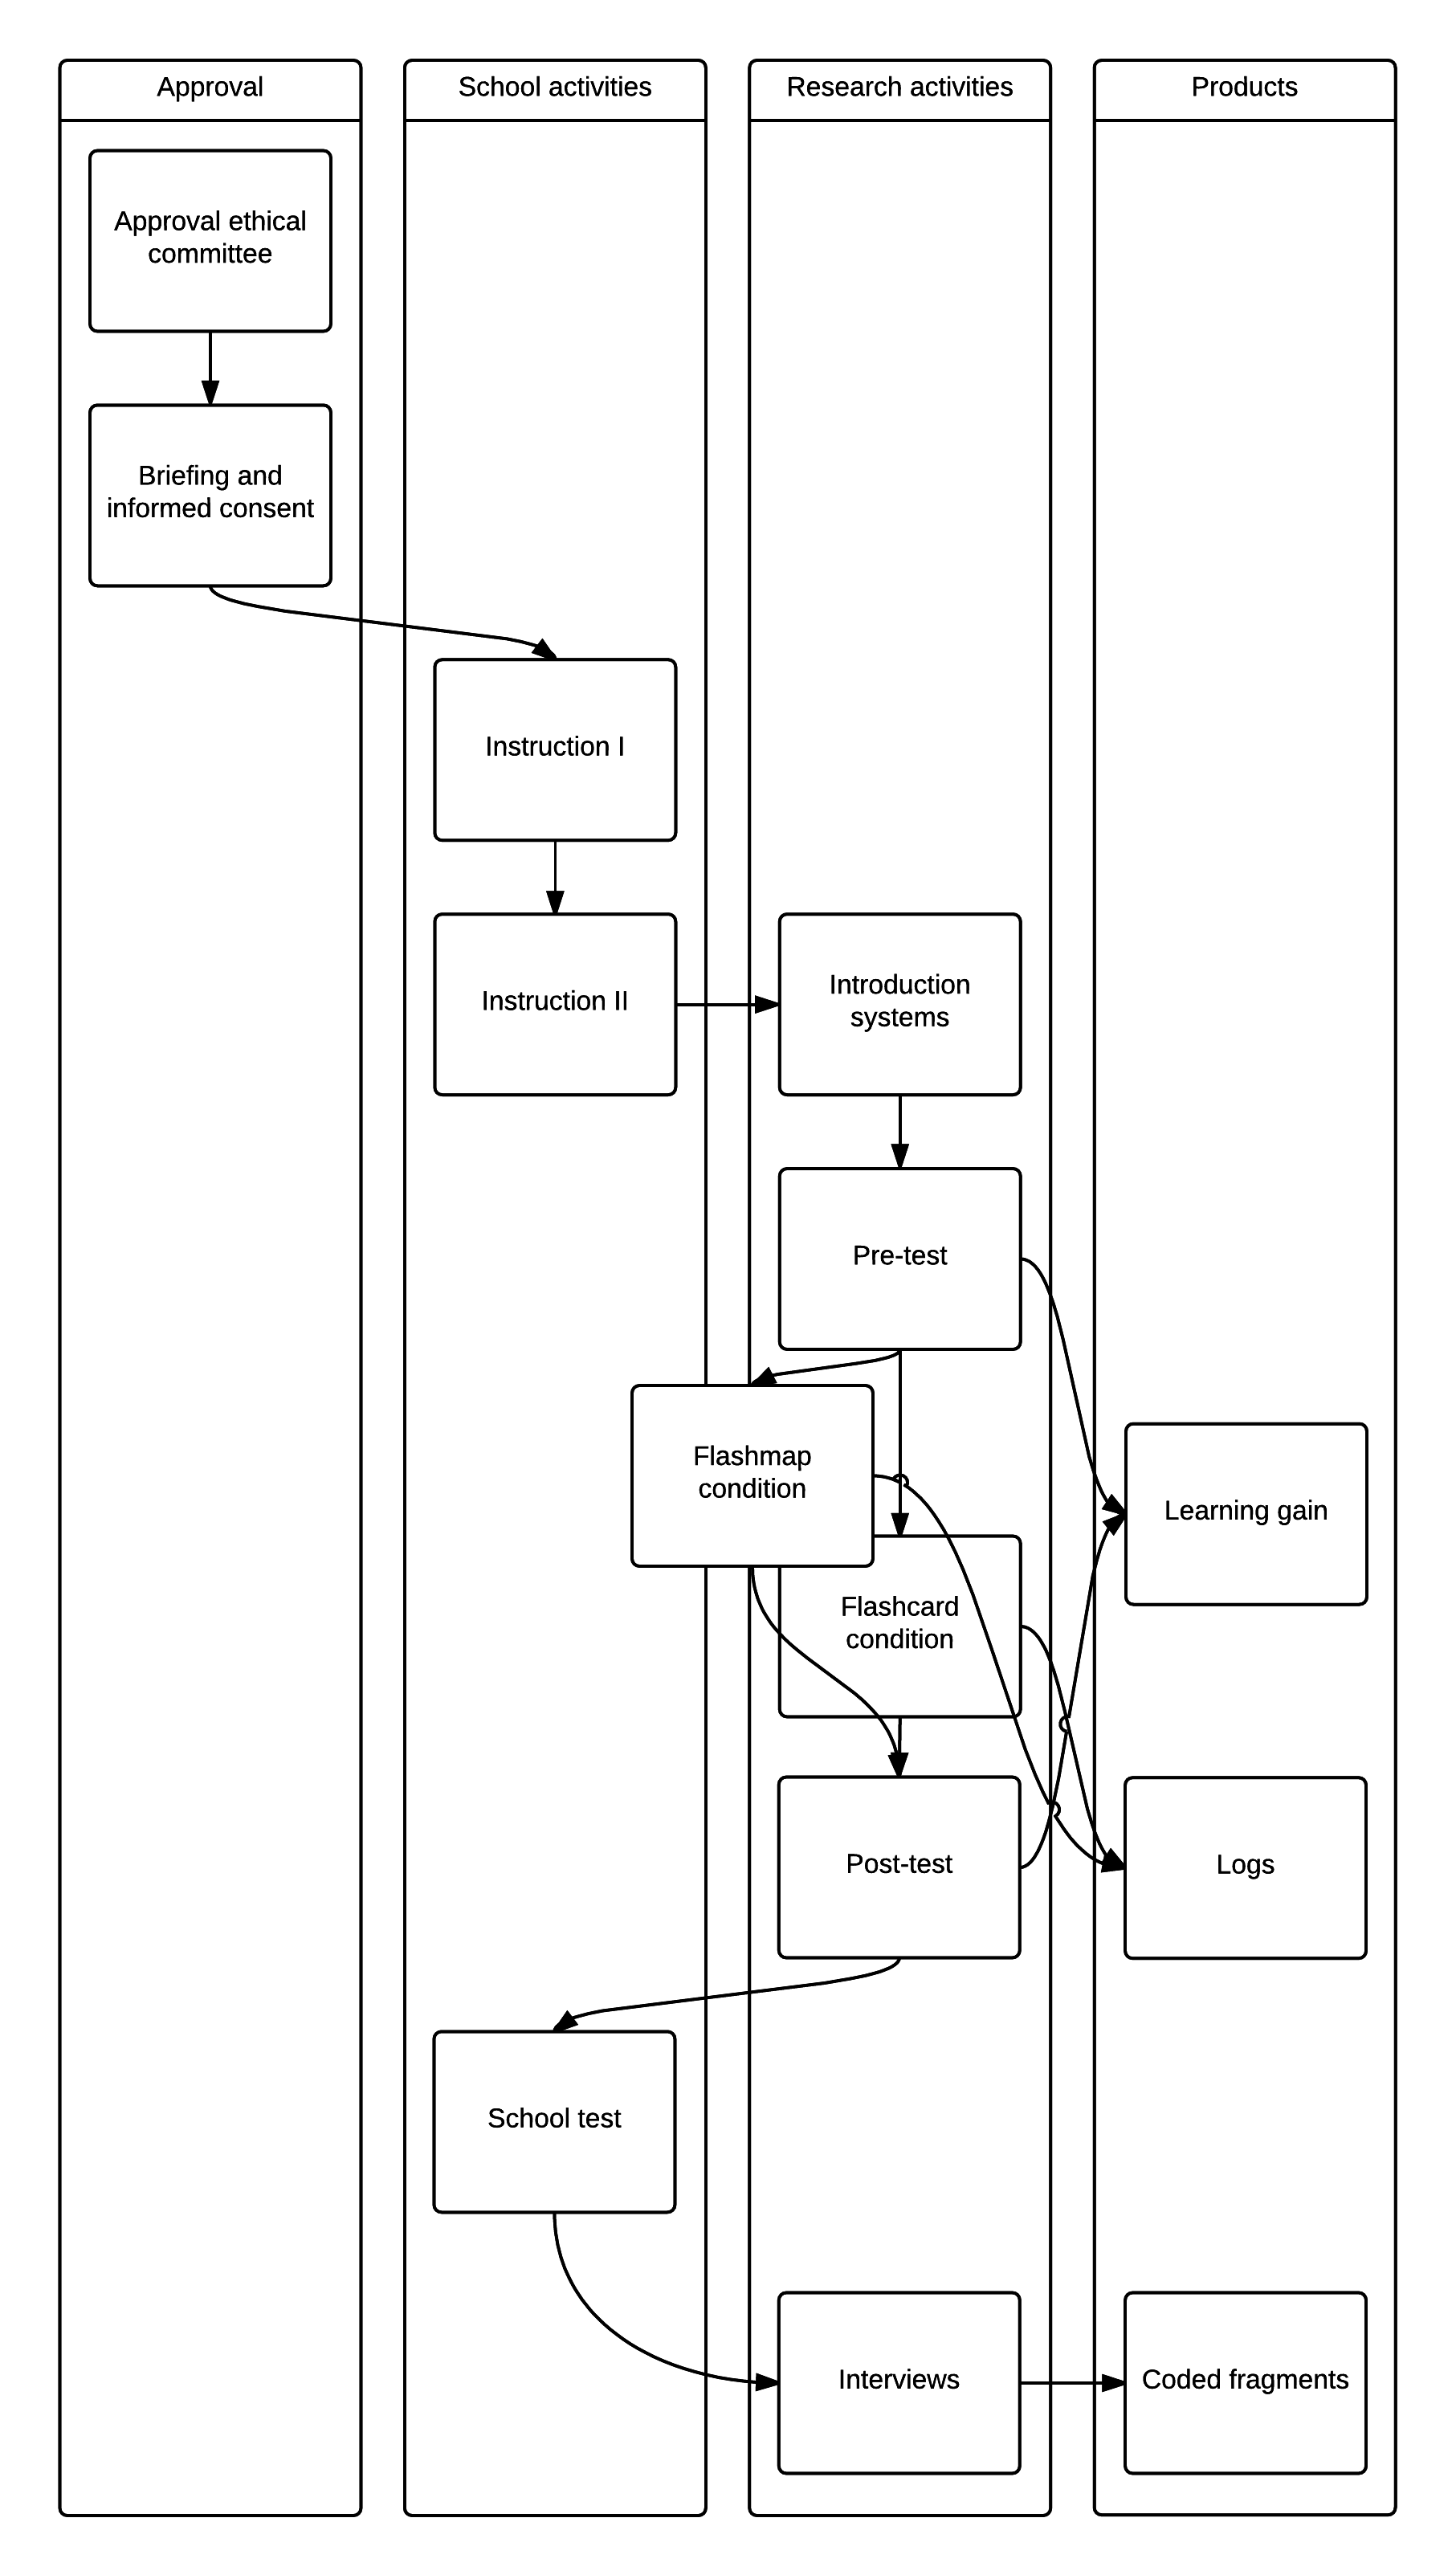
\includegraphics[height=.85\textheight]{img/procedure}
    \caption{An overview of the different steps conducted within the research procedure}
    \label{fig:procedure}
\end{figure}

\section{Data Analysis}

%Describe the type of data you will generate (qualitative, quantitative, mixed-method) and the methods you intend to use to analyze your data. Make sure this fits with your research design and questions. Here you may also address reliability checks for your instrumentation.

Research questions~\ref{benefit}\ref{effectiveness}, \ref{efficiency}, \ref{perception}\ref{usefulness}, and \ref{ease} will be assessed by means of a t-test, using the following hypotheses: 

\begin{tabular}{l l l}
\ref{benefit}\ref{effectiveness} & H0: & $LG_{fc} \leq LG_{fm}$ \\
                                 & Ha: & $LG_{fc} < LG_{fm}$ \\
\ref{benefit}\ref{efficiency}    & H0: & $LGC(fg) \leq LG_{fm}$ \\
                                 & Ha: & $ LGC_{fc} < LG_{fm}$ \\
\ref{perception}\ref{usefulness} & H0: & $U_{fc} \leq U_{fm}$ \\
                                 & Ha: & $U_{fc} < U_{fm}$ \\
\ref{perception}\ref{ease}       & H0: & $E_{fc} \leq E_{fm}$ \\
                                 & Ha: & $E_{fc} < E_{fm}$ \\
\end{tabular}

\noindent where LG = learning gain, LGC = controlled learning gain, U = perceived usefulness, E = perceived ease of use, fc = flashcard condition and fm = flashmap condition. For determining the learning gain, the pre- and post-test have to be scored with a predetermined rubric. The answers will be scored without the scorer being aware whether the question was asked within the pre- or the post-test, or which participant filled in the answer. After both the teacher and the researcher have scored a sample of the answers, the inter-rater reliability will be calculated. The rest of the answers will be scored by the researcher only, and after scoring all of the items the reliability of test items will be assessed further using Item Response Theory.

The interviews will be transcribed and coded according to \citeA{baarda}, and another inter-rater reliability will be determined by a sample of the interviews coded by the researcher and a peer researcher. The coded fragments will be checked to validate the results from the t-tests, together with the server logs made during the experiment.

\chapter{Planning}

\section{Timeline}

%Include an overview for whole project

Table~\ref{tab:planning} displays the activities together with the intended week number of execution and generated outputs. 

\setcounter{table}{0}

\begin{table}
    \begin{tabular}{ l | p{.4\textwidth} | p{.4\textwidth}}
        \centering
        \textbf{Week nr} & \textbf{Activity} & \textbf{Outputs} \\ \hline
        16 & Request approval ethical committee & Approval ethical committee \\ \hline
        17 & Finalising concept map & Concept map \\ \hline
        17 & Finalising flashcards & Flash cards \\ \hline
        17 & Finalising item bank questions & Item bank questions \\ \hline
        18 & Finalising adaption Technology Acceptance Model questionnaire & Adapted Technology Acceptance Model questionnaire \\ \hline
        18 & Evaluation concept map with teacher & Improved concept map \\ \hline
        18 & Evaluation flashcards with teacher & Improved flashcards \\ \hline
        18 & Evaluation item bank questions with teacher & Improved item bank questions \\ \hline
        19 & Finalising software & Flashcard and Flashmap software \\ \hline
        19 & Briefing and informed concent & Approval parents and children \\ \hline
        19 & Instruction I & \\ \hline
        20 & Instruction II & \\ \hline
        20 & Introduction flashcard and -map systems to students & \\ \hline
        20 & Pre-test & Initial answers \\ \hline
        20 & Experiment & User data \\ \hline
        21 & Post-test & Final answers \\ \hline
        21 & Questionnaire & Perceived usage and ease of use \\ \hline
        21 & Finalise scoring sample items & Scored sample items \\ \hline
        22 & School test & \\ \hline
        23 & Interviews & Audio conversations \\ \hline
        23 & Determine inter-rater reliability with teacher & Cohen's kappa \\ \hline
        25 & Finalise scoring all items & Scored items \\ \hline
        27 & Finalise transcribing interviews & Transcribed interviews \\ \hline
        28 & Finalise coding interviews & Coded fragments \\ \hline
        29 & Perform t-tests & Quantitative results \\ \hline
        32 & Finalising report & Research report \\
    \end{tabular}
    \caption{The intended planning for research activities and outputs during this project \label{tab:planning}}
\end{table}

\section{Outputs}

%Include descriptions and target dates for final outputs (e.g., advice reports, delivery of products, scientific article) as well as those along the way (e.g. literature review; instruments; data collection).

Their are several products being developed and data being collected during the project. First of all, a concept map will be developed containing the main concepts on 17th century Dutch literature, which will be the basis for the flashcards and the item bank questions. Furthermore, software will be developed being capable of both providing flashcards and flashmaps. The data being collected includes initial and final student answers, questionnaire results audio conversations, and server logs from the interviews, which will then be used for conducting the t-tests and triangulation and expansion purposes. This will finally be documented in the research report.

\bibliographystyle{apacite}
\bibliography{references}
\thispagestyle{fancy}

\end{document}
